\def\year{2015}
\documentclass[letterpaper]{article}
\usepackage{aaai}
\usepackage{fixbib}
\usepackage{times}
\usepackage{helvet}
\usepackage{courier}
%\usepackage[dvipdfmx]{graphicx}
\usepackage{graphicx}
\usepackage{amsmath}
\usepackage{amsfonts}
\usepackage{url}
\frenchspacing
\setlength{\pdfpagewidth}{8.5in}
\setlength{\pdfpageheight}{11in}
\pdfinfo{
/Title (Insert Your Title Here)
/Author (Put All Your Authors Here, Separated by Commas)}
\begin{document}
%
\title{Bayesian Optimization for Crowd Density Prediction}
\author{CS4246 Project: Planning and Decision Making in the Real World  \\ \\
{\bf Team 04} \\
Huang Wei Ling, A0101200R\\
Nathan Azaria, A0113011L\\
Ng Hui Xian Lynnette, A0119646X\\
Nguyen Duc Thien, A0093587M\\
Oh Shunhao, A0065475X\\
}
\maketitle
\begin{abstract}
\begin{quote}
Crowd density prediction is relevant to tackle issues in events such as resource management. Event space is usually limited and there are many concurrent activities at any point of time. Therefore, crowd density prediction is useful for the event committee to plan the layout and schedule of the programs in an event effectively and allows participants of the event to move around the event space efficiently so that they gain most out of attending the event. \\

In this report, we illustrate the use of Bayesian Optimization to find a set of reference points at significant points in an area. For each data point, we compute the shortest path distance from the data point to each of the reference points and used it for GP regression to predict the crowd densities.
\end{quote}
\end{abstract}

\section{Introduction}
In this report, we propose the use of Bayesian Optimization for crowd density prediction. Particularly, we discuss how Bayesian Optimization is used to find a set of reference points in an area for crowd density prediction, how we conduct training on the set of reference points chosen to find the optimal set of reference points that minimises the function $f$ as well as the important requirements of our proposed application. \\

We will touch on the technical details which includes how we compute the shortest path, modelling the distance using GP regression, density and error computations. We will also outline the experimental plan we used to perform and evaluate the performance of Bayesian Optimization for crowd density prediction. \\

The rationale behind using Bayesian Optimization for crowd density prediction is to minimise the error by predicting whether a set of reference points given an environment setup is suitable to predict the crowd density in the environment.

\section{Crowd Density Prediction}

Bayesian Optimisation method is used to predict the crowd density by using a set of $3$ reference points from a known environment. In this section we describe the details of the use of Bayesian Optimization, to later present details on the specific algorithm for calculating the shortest paths and the use of GP regression in the implementation of the function $f$ in Bayesian Optimization.

\subsection{Processing of data}

For our proposed application, we are using a set of 100 locations of people to train the set of reference points selected. First, we divide the set of 100 data into groups of 10. Each group is used together with the set of reference points to compute the shortest path distances and modelled using GP regression to predict the crowd density of 100 people. Then, we can compute the error of the prediction with the set of 100 locations of people and output this result to the Bayesian Optimization process to pick a new set of reference points which are more optimal than the previous set for training.

\subsection{Bayesian Optimization}

In general, the main objective of Bayesian Optimization is to find the optimal (maximum or minimum) of an unknown and costly $x$ to evaluate function $f$, which is to find $x^* = \text{argmax}_x f(x)$ or $x^* = \text{argmin}_x f(x)$. \\

In our proposed application of crowd density prediction, we are interested to minimise the function $f(x)$, which $f(x)$ refers to the error of the crowd density prediction. The $x$ in the function $f(x)$ refers to the input points $c_1, c_2, c_3$ which each of the input points is represented by the $x$ and $y$ coordinates of a location in the floor plan provided.   



\subsection{Important Requirements}

An important requirement of our task is we must have the floor plan in order to perform Bayesian Optimisation for shortest path prediction. Our experiment uses 2 different floor plans from the same event which we apply Bayesian Optimization to each floor, thus assuming statistical independence between the different floors.\\

However, the actual coordinates are likely to have a significant correlation and structure. Thus, one possible improvement is to construct GP models with correlated output, by passing the independent GP priors through a function, such as multi-class classification, as described in a paper by {\it Antoni B.Chan} on the topic of Multivariate Generalized Gaussian Process Models. \\

As we use time-series data for the Gaussian Process, there are potentially a large amount of data points, especially for time periods that last multiple days. Thus the efficiency of the algorithm is important. As we construct separate Gaussian Distributions for each person, the computations can be distributed over multiple machines.


\section{Technical Approach}



\subsection{Generating Shortest Path Coordinates}

We note that in the original data, the positions of each individual at any point of time is given in Cartesian coordinates $(x,y)$. The first step is thus to convert the existing Cartesian coordinates of each person's location specified in the data into a 3-tuple of shortest-path coordinates, $s_1, s_2, s_3$, referring to the shortest paths from the current position to each of the three reference points respectively.\\

\begin{figure}[!h]
  \centering
    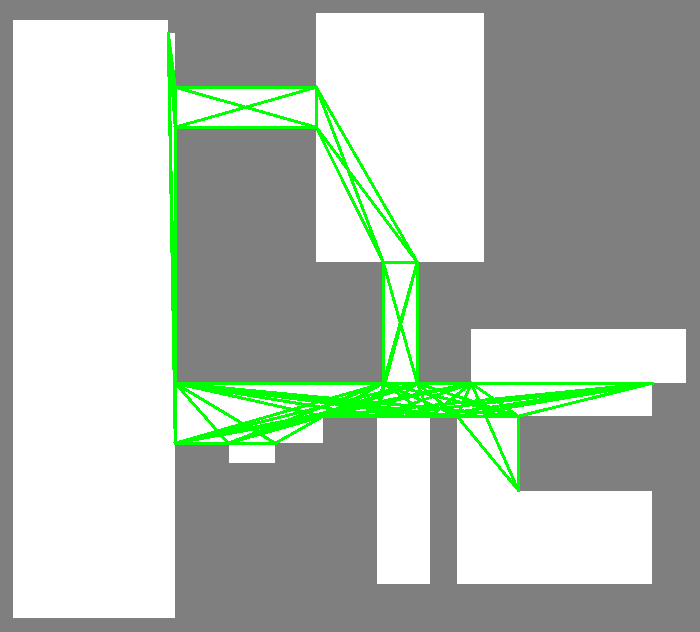
\includegraphics[width=170px]{diagrams/floor18visibilitygraph.png}
  \caption{Visibility Graph generated over the 18th floor of the XXXX building}
  \label{fig:floor18vg}
\end{figure}

Shortest path coordinates are computed using Any-Angle Pathfinding algorithms on grids. A floorplan of the area is used, and abstracted into a grid of blocked and unblocked tiles, representing impassable and passable areas in the actual space respectively. Then, for each $(x,y)$ coordinate in the data, we map it to the nearest unblocked tile on the grid. This can be done efficiently using Kd-trees.\\

\begin{figure}[!h]
  \centering
    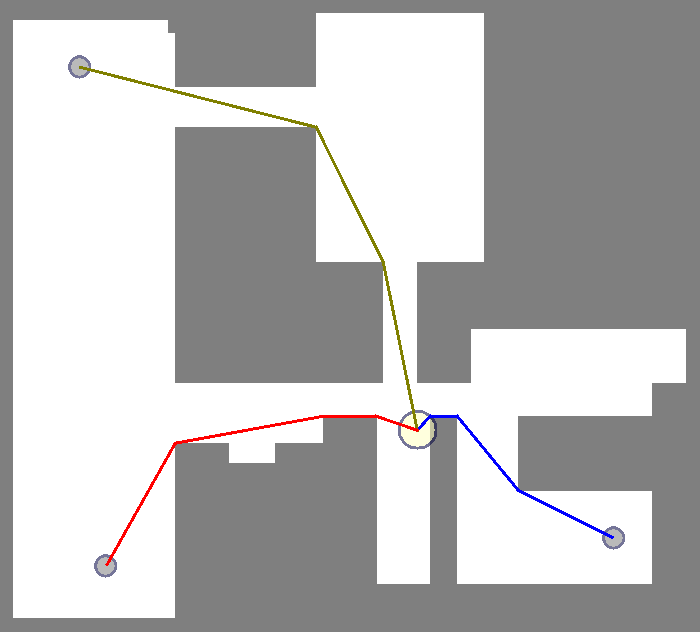
\includegraphics[width=170px]{diagrams/floor18shortestpaths.png}
  \caption{Shortest any-angle paths computed from a single point to three different reference points.}
  \label{fig:floor18sps}
\end{figure}

We then apply an optimal any-angle pathfinding algorithm to compute the shortest path from the $(x,y)$ coordinate to each of the three reference points. This generates three shortest-path queries for each user position. This shortest path computation can be done efficiently as a batch, on an approximately 100x100 grid by preprocessing a visibility graph like shown on Figure \ref{fig:floor18vg}, which can be reused to process each of the shortest path queries (Figure \ref{fig:floor18sps}). Running the A* algorithm on visibility graphs is an optimal offline algorithm for Any-Angle Pathfinding.\footnote{Visibility graph algorithm \url{https://github.com/Ohohcakester/Any-Angle-Pathfinding}}\\

Thus for each point, as there are three reference points, we obtain three shortest-path coordinates, $s_1, s_2, s_3$.

\subsection{Gaussian Processes for Probability Distributions}

Instead of applying the Gaussian Processes to the Cartesian coordinates as before, we apply it to the shortest-path coordinates, $s_1, s_2, s_3$, over time. Similar to before, the shortest path coordinates are modelled as a time series, and each of the three coordinates are regressed independently over time using the Gaussian Process model.\\

The hope is that with a good selection of reference points, the coordinates $s_1, s_2, s_3$ can be regarded as independent of each other without a significant loss of accuracy. From the regression, we obtain, at each point of time, a probability distribution of each of the coordinates $s_1, s_2, s_3$, described as a trivariate normal distribution $\mathcal{N}\tilde (\boldsymbol{\mu},\sigma^2)$.

\subsection{Crowd Density Computation}

The use of shortest-path coordinates over Cartesian coordinates makes density computation more challenging. One can no longer simply select an arbitrary region (e.g. a rectangle) and integrate the probability distribution over all $x$ and $y$ values that fall within the region. One cannot even assume a one-to-one mapping between the shortest-path coordinates and the Cartesian coordinates. \\

Thus the integration has to be carried out differently. Instead of picking a rectangle in the Cartesian plane, we integrate over rectangles defined over the shortest-path coordinates. A rectangle is defined as the set
\[\{(s_1,s_2,s_3) : a_1\leq s_1\leq b_1, a_2\leq s_2\leq b_2, a_3\leq s_3\leq b_3\}\]
for some boundary values $a_1,b_1,a_2,b_2,a_3,b_3 \in \mathbb{R}$.\\

\begin{figure}[!h]
  \centering
    
\includegraphics[width=170px]{diagrams/sprectangles.png}
  \caption{Illustration of the rectangles defined by shortest path coordinates, where $k_1 = k_2 = k_3 = 5$. Each colour corresponds to a different rectangle.}
  \label{fig:sprectangles}
\end{figure}

To define the rectangles, we first note that for each shortest-path coordinate $s_i$, $i \in \{1,2,3\}$, $s_i$ lies within some bounded interval $[0,D_i]$, for some $D_i > 0$. We then divide this interval into $k_i$ intervals of equal length. Interval $j$, where $j \in \{0,1,\cdots,k_i-1\}$ would correspond to the interval $[\frac{j}{k_i}D_i, \frac{j+1}{k_i}D_i]$.\\

Thus we define $\prod_{i=1}^3 k_i$ rectangles, each corresponding to a selection of intervals. For example, the rectangle indexed by the tuple $(0,2,1)$ would refer to $[0,\frac{D_1}{k_1}]\times [\frac{2D_2}{k_2},\frac{3D_2}{k_2}]\times [\frac{D_3}{k_3},\frac{2D_3}{k_3}]$. An illustration of what the rectangles look like in the original map is shown in Figure \ref{fig:sprectangles}.

\subsection{Error Computation}


\subsection{Additional Insights}


\subsection{Improvement}



\section{Experimental Evaluation}



\subsection{Real-World Dataset}

We test our approach using a Attendee Meta-Data (AMD) Hope RFID Dataset from which data is collected from 1224 hackers attending The Last HOPE Conference from 18-20 July 2008, located in Hotel Pennsylvania, New York City.\\

The data set details the location of the attendees through the use of RFID badges that uniquely identify and track them across the conference space over the course of the conference. A plot of one of the position data over time of one of the attendees is shown in Figure .\\


This dataset was used as it has some convenient properties which allow us to construct an experiment to test our model. Firstly, the position data is usually taken at regular intervals of about $30$ seconds apart. Secondly, the data provided is exhaustive (as each attendee to the conference is tagged). \\

This provides enough information to find the actual number of people in each region at any point of time, by simply counting the number of people within the region, within in a time window of $[t-15,t+15)$, where $t$ is the target point of time.

\subsection{Experimental Setup}



\section{Conclusion}



\section{6. Main Roles of Each Member}
\begin{itemize}
\item \textbf{Wei Ling}: 
Writing of the report, keeping track of requirements, and research.
\item \textbf{Nathan}: 
Setting up of the experiment and running the tests using the dataset.
\item \textbf{Lynnette}: 
Setting up and experimenting with the various libraries and available tools, and fine-tuning the Gaussian Process models
\item \textbf{Thien}: 
Setting up and experimenting with the various libraries and available tools, and fine-tuning the Gaussian Process models
\item \textbf{Shunhao}: 
Problem formulation and modelling, mathematics, creating the visualisations and experiment, and writing the report.\cite{manning_introduction_2008}
\end{itemize}

\bibliographystyle{aaai}
\bibliography{report}

\end{document}
